\section{Commentary on the Case Studies}
\label{sec:case-studies}

For further evaluation of the artifact, we invite the reader to take a
tour of FCSL and explore particular example programs that we have
verified. The most convenient way to do it is to use GNU Emacs (or
Aquamacs in OS X) with the installed Proof General
mode\footnote{\url{https://github.com/emacsattic/proofgeneral}} for
interactive proof construction in Coq. Opening any \code{.v}-file in
the editor (use \code{Ctrl-X Ctrl-F} to navigate with Emacs) will
automatically trigger the Proof General mode, making it possible to
``step'' through the file and examine intermediate steps of the
proofs. Note, that in order to step through a particular file in Proof
General, you will need to have all its dependencies (typically listed
as \code{Require Import} arguments at the head of a file) compiled,
which could be done in the case of FCSL via the supplied
\code{make}-script (see~\S \ref{sec:building-project}).


Stepping through a Coq file in Emacs/Proof General can be performed
via the \code{Ctrl-C Ctrl-Enter} shortcut, which makes the interactive
proof engine to process the file till the current position of the
caret. Use \code{Ctrl-C Ctrl-C} to interrupt the interpretation
process (when some part of the buffer remains colored light-red). A
typical Emacs/Proof General layout\footnote{The standard layout is the
  ``{smart}'' one, but different configurations of the buffers can be
  chosen through the \textsf{[Coq] $\rightarrow$ [3 Windows mode
    layout]} menu.} for interactive proof construction is shown in
Figure~\ref{fig:pg}. Use \code{Ctrl-C Ctrl-L} to restore the initial
layout.

\begin{figure*}[t!]
\centering
%
{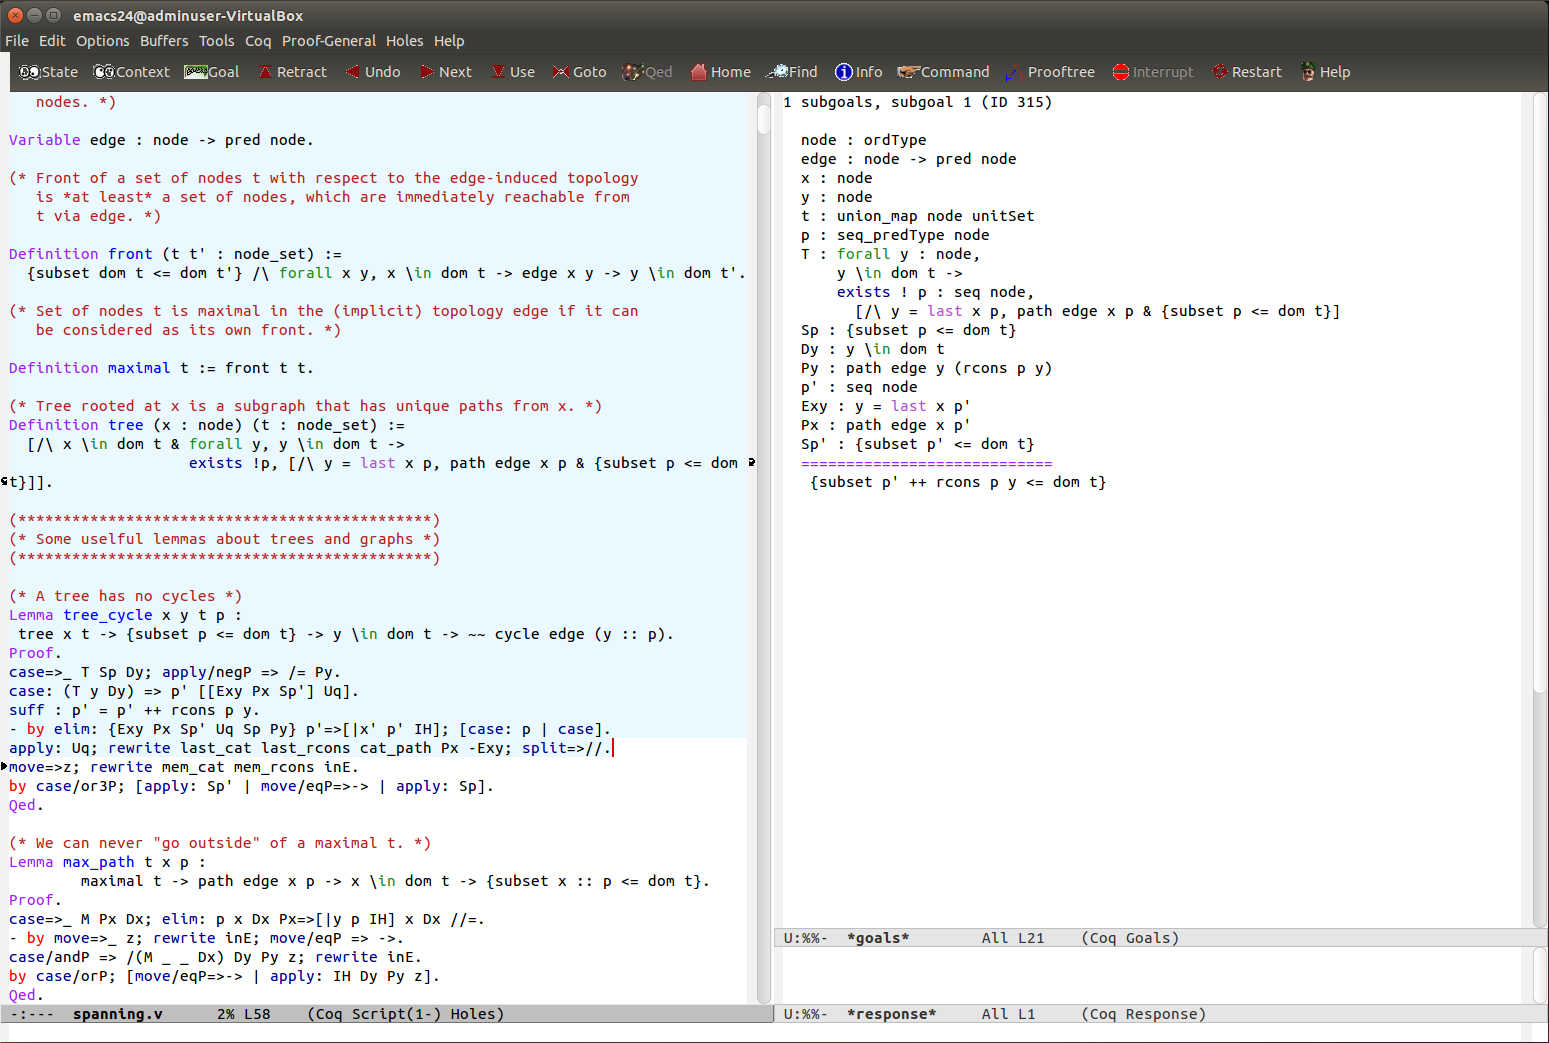
\includegraphics[width=0.96\textwidth]{pg-screen.png}}
%
\caption{The hybrid layout of the Proof General mode in GNU Emacs 24
  (in Ubuntu Linux 14.04) processing the \code{spanning.v} file. The
  left buffer indicates the current file, in which the blue part has
  been already processed by the Coq interactive interpreter. The
  top-right buffer displays the current proof context (above the
  \textcolor{violet}{\texttt{\small{=======}}} line) and the goals
  remaining to be proved. The bottom-right buffer shows the responses
  of the interpreter.}
\label{fig:pg}
\end{figure*}

\subsection{Basic examples}
\label{sec:basic-examples}

Folder: \texttt{Examples/Basic}

\subsubsection{Locking structures (\code{locks.v})}
\label{sec:locks}

Locks are the simplest fine-grained concurrent data structures, and we
have implemented two instances of the locking mechanism: a CAS-based
spinlock and a ticketed lock. The file \code{locks.v} defines a
uniform basic structure for locks by packaging a number of values and
facts about them in a dependent record as follows:

\begin{lstlisting}
Structure lock_info := LockInfo {
  label_of: nat;
  pcm_of : encoded_pcm; 
  inv_of : pcm_of -> Pred heap; 
  precise_of : forall g, precise (inv_of g)
}.
\end{lstlisting}

The structure's fields are the label \code{label_of} of a concurroid
implementing the lock; the client-specific PCM \code{pcm_of},
specifying the nature of the contributions that separate threads
perform over the lock-protected part of the heap; the \emph{lock
  invariant} \code{inv_of} that relates the cumulative contribution of
all the threads and the heap, which is protected by the lock, and the
proof \code{precise_of} that the invariant is \emph{precise}, which is
crucial for the consistency of the locking protocol in the classical
Concurrent Separation Logic~\cite{OHearn:TCS07}.
%

\paragraph{Abstract specification of a lock.~~}

What is a suitable abstract specification for a locking structure? To
answer this question, we adopt the idea of specifying concurrent data
structures via \emph{abstract
  predicates}~\cite{DinsdaleYoung-al:ECOOP10} and provide a lock
interface in the form of two abstract procedures: \code{lock} and
\code{unlock}. Every data structure, implementing the lock protocol,
will require to provide the implementation of these procedures. The
lock interface is parametrized by two abstract predicates,
constraining some part of the state: \code{is_lock} and
\code{locked}. The former denotes the fact that the part of state
implements belongs to the locking protocol, while the latter one
identifies that the lock is currently being locked by the current
thread.

Both predicates should satisfy a number of axioms, which are packaged
into a dependent record in the section \code{LockStruct} (where the
predicates are referred to as \code{locked_op} and \code{is_lock_op}).
For instance, the following axiom expresses the lock's mutual
exclusion property:

\begin{lstlisting}
forall s gl ge, locked_op gl ge s -> locked_op ge gl (transp s)-> False  
\end{lstlisting}

Specifically, it states that the situation when lock is held by the current
thread (\code{locked_op gl ge s}) \emph{and} it is simultaneously held
by some other thread, which is expressed via a \emph{transposition} of
a concurroid's state \code{s} (\code{locked_op ge gl (transp s)}),
implies the falsehood. The other property implies that if the state
represents a locked lock, it also corresponds to a resource, which
belongs to the lock protocol:

\begin{lstlisting}
forall s gl ge, locked_op gl ge s -> is_lock_op gl ge s  
\end{lstlisting}

These two predicates serve as parameters to specifications
\code{lock_spec} and \code{unlock_spec}, which are supposed to be
fulfilled by the locking and unlocking procedures,
correspondingly. Let us consider the specification for locking,
defined as follows:

\begin{lstlisting}
Definition lock_spec is_lock locked : spec unit := 
  (* precondition predicate *)
  (fun i => exists (hl he : heap) (gl ge: U) i', 
     i = hp ->> [hl, tt, he] \+ i' /\ is_lock gl ge i', 
   (* postcondition predicate *)
   fun i y m => forall hl he (gl ge: U) i', 
     i = hp ->> [hl, tt, he] \+ i' -> is_lock gl ge i' ->
     exists h ge' he' m',
       [/\ m = hp ->> [hl \+ h, tt, he'] \+ m', 
           locked gl ge' m',
           valid (gl \+ ge') & I (gl \+ ge') h]).
\end{lstlisting}

The specification \code{lock_spec} takes predicates \code{is_lock} and
\code{locked} as parameters. It states that the return type of the
locking procedure is \code{unit}. While reminiscent to the
specifications, shown in \S \ref{sec:spanning-tree} for the spanning
tree procedures, this spec bears two significant differences that are,
in fact, typical rudiments from the earlier stages of FCSL
development.

\begin{itemize}

\item \emph{\textbf{Explicit concurroid structure}}: The concurroid
  states in the pre- and postconditions are specified explicitly. For
  instance, the thread-local state concurroid is denoted as \code{hp
    ->> [hl, tt, he]}, where \code{hp} is its label, \code{hp} and
  \code{he} are heaps, that belong to this thread and its environment,
  correspondingly, and \code{tt} is its joint component, which is of
  \code{unit} type. With getters, which were developed later, we would
  be able to write the same part of the assertion as \code{pv_self i =
    hl /\\ pv_other i = he} (actually, we could avoid mentioning
  \code{he} at all, since it is irrelevant in this case).


\item \emph{\textbf{Binary postconditions}}: Unlike the postconditions
  in the specs we've seen before, the postcondition of \code{lock_spec}
  is \emph{binary}, as it relates the pre-state \code{i} with a result
  \code{y} and the post-state \code{m} (the ``unary'' postconditions
  typically constrain just the result and the post-state). Binary
  postconditions are useful to capture the essence of logical (or,
  \emph{ghost}) variables, that serve for the purpose of relating the
  pre- and postconditions~\cite{Nanevski-al:POPL10}. For instance, the
  binary postcondition in \code{lock_spec} states that the
  thread-local heap, which initially was \code{hl}, at the end of the
  locking procedure became \code{hl \\+ h}, \ie, the heap \code{h} was
  acquired by the thread. With the notation for logical variables,
  used in the spanning tree example, we could have expressed the same
  relation by making \code{hl} to be a logical variable stated in the
  preamble of the specification as~\code{\{hl ...\}}.
\end{itemize}

We can now read the specification \code{lock_spec}. In plain words, it
postulates that the pre-state, observed by the thread can be split
into two concurroids: the one for thread-local heaps (labelled
\code{hp}), and another abstract concurroid for a lock (\code{i'}),
such that \code{is_lock gl ge i'} holds and \code{gl}, \code{ge} are
the contributions of this and other threads to the lock-protected
resource, correspondingly. At the end of the locking procedure, the
thread-local heap in the post-state \code{m} has been augmented by the
heap \code{h}, released by the lock. Moreover, the lock is now in the
locked state, which is captured by the predicate \code{locked gl ge'
  m'}, constrining the state \code{m'}, which belongs to the lock
Finally, the acquired heap satisfies the lock-specific invariant
\code{I (gl \+ ge')}, which we can now use for local reasoning.


We next instantiate the general locking data structure for two
specific locking protocols and instantiate abstract predicates
\code{is_lock} and \code{locked} for them.

\subsubsection{CAS-lock (\code{caslock.v})}
\label{sec:cas-lock}

The intuition behind the CAS-based lock protocol is described in detail
in the original FCSL paper~\cite{Nanevski-al:ESOP14}, which uses it as
a running example.

The implementation of the lock first refines the general lock
structure \code{lock_info} from \code{locks.v} by adding one more
parameter: an address of the ``flag pointer'', which holds the boolean
value indicating the fact of locking:

\begin{lstlisting}
Structure lockT := LockT {
  lock_info_of :> lock_info;
  lock_of : ptr 
}.  
\end{lstlisting}

The coherence predicate describes the valid states of the lock, which
are either ``locked'' (the protected heap is gone, the locking flag is
\code{true}) or ``unlocked'', in which case the lock concurroid has
the protected heap \code{h} in each joint state, and the heap
satisfies the client-provided precise invariant.

\begin{lstlisting}
Definition validRes s :=
  exists (mL mE : lift mutexUnlifted) (gL gE : U) (b : bool) h,
    s = l ->> [(mL, gL), lk :-> b \+ h, (mE, gE)] /\ P (mL \+ mE) (gL \+ gE) b h.

Definition cohRes P := [Pred s : state | [/\ validH s, validSO s & validRes P s]].

Definition locked m (g : U) b (h : heap) := [/\ m = up own, b = true & h = Unit].
Definition unlocked m g b h := [/\ m = up nown, b = false & I g h].
Definition either m g b h := locked m g b h \/ unlocked m g b h.

Definition coh := cohRes either. 
\end{lstlisting}

The definition of the CAS-lock coherence predicate (section
\code{LockCoh}) includes the proofs of the standard concurroid
axioms, already mentioned in \S \ref{sec:spanning-tree}.

In addition to trivial (\ie, identity-like) internal transitions, the
lock concurroid features external transitions implementing
communication via heap ownership transfer. In particular, the
\emph{acquire} transition (described in detail in~\cite[\S
4]{Nanevski-al:ESOP14}) corresponds to the lock concurroid getting a
heap satisfying the invariant \code{I (gL' \+ gE)} and placing it to
its own joint component, as defined by the following relation between
the initial and the final states (\code{s} and \code{s'},
correspondingly):\footnote{At the moment of implementing the locking
  protocols, the machinery for state getters (see the file
  \texttt{getter.v}) hasn't yet been implemented, which is why the
  definitions of concurroid states and transitions look a bit
  different from those of the spanning tree example. For the same
  reason, the proofs of the lemmas about locks are significantly
  larger, as they haven't been optimized using getters.}

%\newpage

\begin{lstlisting}
Definition acq_rel s s' :=  
  exists gL gL' gE : U, 
    [/\ s  = l ->> [(up own, gL), lk :-> true, (up nown, gE)],
        s' = l ->> [(up nown, gL'), lk :-> false \+ h, (up nown, gE)],
        valid (gL' \+ gE), valid (lk :-> false \+ h) &
        I (gL' \+ gE) h] /\ s \In coh.  
\end{lstlisting}

Simultaneously, the value of the flag pointer \code{lk} is being
changed from \code{true} to \code{false} and the value of the
\emph{mutex auxiliary resource} changes from \code{(up own)} to
\code{(up nown)} in the self-part, indicating that the lock is no
longer held by this thread.

The \emph{release} transition is symmetric and corresponds to the lock
giving up ownership on the heap \code{h} from its joint part,
simultaneously with changing the value of the flag pointer, but
preserving the value of the client specific auxiliary value~\code{gL}:

\begin{lstlisting}
Definition rel_rel s s' :=  
  exists gL gE : U, 
    [/\ s  = l ->> [(up nown, gL), lk :-> false \+ h, (up nown, gE)],
        s' = l ->> [(up own, gL), lk :-> true, (up nown, gE)] & 
        s \In coh].  
\end{lstlisting}

The two defined transitions form a \emph{communication channel}, such
the heap may be transferred through it. Together with the coherence
predicate, the transitions are next packaged in the definition of the
concurroid \code{CLock} at the end of the \code{Exports} section of
the \code{LockGuar} module.

Next, we define so-called \emph{pre-actions}, which implement the
machinery of the corresponding acquire/release transitions of the lock
concurroid, connecting it to the operational semantics of machine
commands, such as \code{CAS} and \code{write}. This is done in the
sections \code{LockReleaseAct} and \code{LockAcquireAct}. Later, the
sections \code{CASAct} and \code{UnlockAct} turn this pre-actions into
full-fledged actions that span a \emph{composite} concurroid
\code{(entangle (Priv hp) (CLock lkT))}, obtained by connecting
acquire/release transitions of its constituents. Following the
transitions with different ``polarity'', such actions perform a
transfer of the heap from the lock's joint state to the thread-local
state (described by the concurroid \code{Priv hp}) and vice versa: see
the definitions of \code{cas_step} and \code{unlock_step}
relations.\footnote{With the introduction of state getters, this
  pattern of defining actions operating with the composite concurroid
  (e.g., \texttt{(entangle (Priv hp) (CLock lkT))}), has been rendered
  obsolete, and such actions are defined directly in the later case
  studies, such as Treiber stack~(\S\ref{sec:treiber-stack}).}

Similarly to the development of the spanning tree concurroid in \S
\ref{sec:spanning-tree} we next give stable specifications to the
atomic actions, operating with the lock state. For instance, the
\code{CAS}-like operation, which, when successful, performs the heap
ownership transfer from the lock-protected state to the thread-local
state is given the following spec (with explicit concurroid structure
and binary posts) in the form of a structural lemma:

\begin{lstlisting}
Lemma val_cas1 (hL hE : heap) (mL mE : lift mutexUnlifted) (gL gE : U) (b : bool) h (r : cont bool) : 
        (* if we succeed *)
        (forall hE' gE' h', 
           valid (gL \+ gE') ->
           I (gL \+ gE') h' ->
           hp ->> [hL \+ h', tt, hE'] \+ 
            l ->> [(up own, gL), lk :-> true, (up nown, gE')] \In Mod.coh V ->
           r true (hp ->> [hL \+ h', tt, hE'] \+ 
                    l ->> [(up own, gL), lk :-> true, (up nown, gE')])) ->
        (* if we fail *)
        (forall hE' mE' gE' (b' : bool) h', 
           hp ->> [hL, tt, hE'] \+ 
            l ->> [(mL, gL), lk :-> b' \+ h', (mE', gE')] \In Mod.coh V ->
           r false (hp ->> [hL, tt, hE'] \+ 
                     l ->> [(mL, gL), lk :-> b' \+ h', (mE', gE')])) ->
        verify (hp ->> [hL, tt, hE] \+ 
                 l ->> [(mL, gL), lk :-> b \+ h, (mE, gE)])
               (act (CAS hp lkT)) r.  
\end{lstlisting}

The first of the two ``continuations'' postulates that in the case of
the success (the result is \code{true}) the heap \code{h'} satisfying
\code{I (gL \+ gE')} has been transferred to the thread-local
state. The second continuation states that in the case of failure the
heap hasn't been transferred, and we don't know anything specific
about it (since it could have been acquired by another thread by that
moment). This weakening is required to make such specification stable.

We then define the actual meaning of the \code{locked} and
\code{is_lock} predicates for the CAS-lock and prove that such
definitions satisfy the axioms, imposed by the abstract lock
structure. The \code{c_is_lock} predicate simply describes that the
part of the state, constrained by it, satisfied the coherence
predicate of CAS-lock:

\begin{lstlisting}
Definition c_is_lock (gl ge : U) s := 
  exists (ml me: lift mutexUnlifted) (b: bool) (h: heap),
    s = l ->> [(ml, gl), flag :-> b \+ h, (me, ge)] /\
    s \In Mod.coh (CLock lkT).  
\end{lstlisting}

The \code{c_locked} predicate makes sure that this thread currently
holds the lock (\ie, its self-component has \code{(up own)} element of
the mutual exclusion PCM):

\begin{lstlisting}
Definition c_locked (gl ge : U) s :=
  s = l ->> [(up own, gl), flag :-> true, (up nown, ge)] /\
  s \In Mod.coh (CLock lkT).  
\end{lstlisting}

Finally, with these two predicates, we can give specifications to the
locking and unlocking procedures of the CAS-lock. Both procedures
operate on the composite concurroid, obtained as an entanglement of
the thread-local state and the concurroid implementing the locking
protocol.

\begin{lstlisting}
Notation W := (entangle (Priv hp) (CLock lkT)).   
\end{lstlisting}

The locking definition is a simple CAS-loop over the locking flag
pointer (which is set using the lock-specific action \code{CAS},
defined and specified earlier in the file):

\begin{lstlisting}
Definition cas_lock_spec : spec unit := @lock_spec hp lkT c_is_lock c_locked.

Program Definition cas_lock_proc : STbin W (cas_lock_spec) :=
 Do (ffix (fun (loop : unit -> STbin W cas_lock_spec) (_ : unit) =>
       Do (b <-- act (CAS hp lkT);
           if b then ret tt else loop tt)) tt).
\end{lstlisting}

The unlocking procedure is a single invocation of the \code{unlock}
action, which is operationally equivalent to writing into the locking
flag. However, in order to invoke it, the current thread should hold
the lock, which is ensured by the precondition:

\begin{lstlisting}
Definition cas_unlock_spec : spec unit := @unlock_spec hp lkT f c_is_lock c_locked.

Program Definition cas_unlock : STbin W (cas_unlock_spec) := Do (act (unlock hp pf)).  
\end{lstlisting}

\subsubsection{Ticketed lock (\code{ticketed.v})}
\label{sec:ticketed-lock}

The ticketed lock (described in detail
in~\cite[Appendix~E]{Nanevski-al:ESOP14}) implements a different
protocol with better fairness guarantees, in which the threads,
competing for the lock, first ``draw'' tickets, allowing them to
request the access to the resource in the ``first-come, first-served''
order.

The ticketed lock augments the generic lock structure \code{lock_info}
by adding two more fields to it:

\begin{lstlisting}
Structure tlockT := TLockT {
  owner_of : ptr; 
  next_of : ptr;
  lock_info_of :> lock_info
}.  
\end{lstlisting}

The field \code{owner_of} stands for the pointer, whose current target
value is the ``counter'', displaying the ticket, the owner of which is
currently being served, or may come and get the lock-protected
resource. The field \code{next_of} defines a pointer, whose target
value is the next vacant ticket to be ``drawn'' by some thread. This
leads to three generic states in which the ticketed lock can be: in
addition to ``locked'' and ``unlocked'' state, there adds a
``transit'' state, meaning that there is a thread, which is just about
to be served, as it has the right ticket, although it hasn't acquired
the resource yet, hence the lock is not yet taken. This results in
the following definition of the ticketed lock's coherence:

\begin{lstlisting}
Definition validDispenser P s :=
  exists (n1 n2 : nat) (fL fE : nat_set) (gL gE : U) (b : bool) (h : heap),     
    [/\ s = dl ->> [(fL, gL), owner :-> (n1, b) \+ next :-> n2 \+ h, (fE, gE)], 
        n1 <= n2 & P n1 n2 (fL \+ fE) (gL \+ gE) b h].  

Definition cohRes P := 
  [Pred s : state | [/\ validH s, validSO s & validDispenser P s]].

Definition locked n1 (f : nat_set) b (h : heap) := 
  [/\ n1 \in dom f, b = true & h = Unit].

Definition transit n1 n2 (f : nat_set) (g : U) b h := 
  [/\ n1 \in dom f, b = false, n1 < n2 & I g h].

Definition unlocked (n1 n2 : nat) (g : U) b h := 
  [/\ n1 = n2, b = false & I g h].

Definition either n1 n2 (f : nat_set) g b h :=
  dom f =i [pred x | n1 <= x < n2] /\
  [\/ locked n1 f b h | if n1 < n2 then transit n1 n2 f g b h else unlocked n1 n2 g b h]. 

Definition coh := cohRes either. 
  \end{lstlisting}

The boolean value \code{b} in the target value of the \code{owner}
pointer in the joint part of the ticketed lock concurroid's state
bears logical meaning, indicating, whether the lock is locked, in order
to distinguish between the \code{locked} and \code{transit} states.
%
The \code{transit} state differs from the \code{unlocked} state, as
the latter assumes no threads waiting to be served (the ticket
\code{n1} of the counter is the same as the ticket \code{n2} at the
dispenser).
%
The self/other parts of the concurroid, besides the client-specific
contributions \code{gL} and \code{gE} contain the sets of currently
held tickets, implemented as finite sets of type \code{nat_set}:
\code{fL} and \code{fE}. Indeed, final sets form a PCM with disjoint
union as an operation. The coherence predicate \code{either} ensures
that all currently held by threads tickets are in the range \code{n1
  <= x < n2}. This design solution is describe in more detail
in~\cite[Appendix~E.2]{Nanevski-al:ESOP14}.

The ticketed lock concurroid features three transitions.
\code{int_rel} describes ``drawing'' of a ticket and
corresponds operationally to a fetch-and-increment
command. Similarly to the CAS-lock, the acquire transition
\code{acq_rel} corresponds to \emph{unlocking} (operationally, this is
just a read command), and the release transition \code{rel_rel}
defines the locking (it changes the value of the logical flag
\code{b}, but operationally can be effectively considered as a no-op).

The layout of defining the actions of the ticketed lock protocol (some
of them, inded, cover the entanglement of the concurroid for the
thread-local state and the one of the ticketed lock, \eg, the
\code{TickTryLockAct} action) follows the same structure as for the
CAS-lock (\S \ref{sec:cas-lock}).

The instances of abstract lock predicates are defined for the ticketed
lock as follows:

\begin{lstlisting}
Definition t_is_lock (gl ge : U) s := 
  exists (fl fe: nat_set) (n1 n2: nat) (b: bool) (h: heap),
    s = l ->> [(fl, gl), owner :-> (n1, b) \+ next :-> n2 \+ h, (fe, ge)] /\ s \In Mod.coh (TLock lkT).

Definition t_locked (gl ge: U) s :=
  (exists (fl fe : nat_set) (n1 n2: nat),
    s = l->>[(fl \+ #n1, gl), owner:->(n1, true) \+ next:->n2, (fe, ge)]) /\ s \In Mod.coh (TLock lkT).  
\end{lstlisting}

In particular, \code{t_locked} requires the logical flag \code{b} to be
\code{true} and the current thread to own the ticket \code{n1}, which
is currently being served. These two facts together make sure that
this thread indeed holds the lock.
%
The locking program first ``draws'' atomically a ticket and then spins
in the loop until this ticket is displayed on the counter (checked by
the action \code{ttryLock}).

\begin{lstlisting}
Program Definition tlock : STbin W (tlock_spec) :=
 Do (n <-- extend _ (act (tdraw lkT)); (* draw a ticket *)
     ffix (fun (loop : unit -> STbin W (t_loop_spec n)) (_ : unit) =>
       Do (b <-- act (ttryLock hp lkT n); (* check the counter *)
           if b then ret tt else loop tt)) tt).
\end{lstlisting}

The derived specification, therefore, conforms to the abstract spec of
locking from \code{locks.v}, instantiated with specific predicates
\code{t_is_lock} and \code{t_locked}. The definition of the unlocking
procedure is straightforward.

\subsubsection{Coarse-grained incrementor (\code{incrementor.v})}
\label{sec:incrementor}

\emph{Incrementor} is a toy coarse-grained concurrent program,
described as a running example for introducing FCSL~\cite[\S
3]{Nanevski-al:ESOP14}. It is a parametrized by a lock structure,
which protects a heap, consisting of a single pointer \code{x},
pointing to a natural number. The concurrent thread can add arbitrary
non-negative amounts to the value, given that it acquires the lock
first, so the pointer's value will be modified in a race-free
manner. These added amounts are ``subjective contributions'', made to
the lock-protected resource by concurrent threads, hence, the
incrementor-specific PCM is a set of natural number with addition as
join operation and zero as a unit element.

The lock invariant for an incrementor is, thus, defined as follows,
stating that the heap is a single entry of the pointer \code{x}, whose
target value is the cumulative contribution \code{g} of the threads,
operating with the resource.

\begin{lstlisting}
Definition incr_inv (g : nat) := [Pred h | h = x :-> g].  
\end{lstlisting}

We next prove that this variant is indeed \emph{precise}, \ie, it
unambiguously picks out an area of heap~\cite{OHearn:TCS07}:

\begin{lstlisting}
Lemma incr_inv_prec (g : [encoded_pcm of nat]) : precise (incr_inv g).
Proof. by move => h1 h2 t1 t2 V1 E; move=>->->. Qed.  
\end{lstlisting}

The incrementor procedure is given specification using the familiar
unary pre- and post-conditions with \code{gs} being a logical
variable, binding the initial amount of self-contribution to the
incrementor resource by this particular thread.

\begin{lstlisting}
Program Definition incr n : 
 {gs}, STsep [W] 
         (fun i => exists sl go,
            i = hp ->> [Unit, tt, pv_other i] \+ sl /\ is_lock gs go sl,
          fun (_: unit) m => exists sl go,
            m = hp ->> [Unit, tt, pv_other m] \+ sl /\ 
            is_lock (gs + n) go sl) :=  
  Do (lock;;
      tmp <-- [priv_read hp nat x];
      [priv_write hp x (tmp + n)];;
      unlock (@pfF n)).  
\end{lstlisting}

The precondition, given in a \emph{small footprint} states that the
local heap is empty (\ie, it is \code{Unit}), and the
self-contribution is \code{gs} (which is captured by the abstract
predicate \code{is_lock gs go sl}). At the end, the local heap is
empty again, but the local contribution has been changed to \code{(gs
  + n)}, which is precisely the subjective effect of the incrementor.

The body of the incrementor procedure first acquires the lock via the
\code{lock} procedure, transferring the pointer to be incremented to
the thread-local heap. It then reads the current pointer's value via
the action \code{priv_read}, defined over the thread-local state
concurroid and ``injected'' into the entanglement via the \code{[...]}
macro. Next, it writes the new value \code{tmp + n} into the pointer
using the \code{priv_write} action. Finally, it unlocks the lock using
the \code{unlock} procedure, which requires a provably \emph{local}
function as an argument. The intuition behind this requirement is defined
in the initial paper on Subjective Concurrent Separation
Logic~\cite{LeyWild-Nanevski:POPL13}. Here, such function (\code{fun x
  => x + n}) is provided by the proof of the following lemma:

\begin{lstlisting}
Lemma pfF n : @local [encoded_pcm of nat] (fun x => x + n). 
Proof. by move=>m y; rewrite /= -addnAC. Qed.
\end{lstlisting}

\subsubsection{Coarse-grained allocator (\code{alloc.v})}
\label{sec:allocator}

A coarse-grained concurrent memory allocator, used by many algoritms
and data structures, is another client of the abstract lock
library. 

The allocator is implemented as a lock-protected chunk of memory,
representing a pool of available entries and mirrored as a logical
list of pointers with a ``sentinel'' pointer, which points to the list
of available entries. The allocation is, therefore, implemented as
taking the first available entry in the pool and moving it logically to the
thread-local state, simultaneously with changing the target value of
the sentinel pointer, so it would point to the next available memory
entry. In the case if the pool is empty, the allocator loops until
some other thread frees memory. The \code{free} operation simply
returns the deallocated memory cell and registers it as a new logical
``head'' of the memory pool.

The allocator's lock invariant is implemented via the two following
definitions:

\begin{lstlisting}
Fixpoint alloc_inv' avl := 
  [Pred h | if avl is x::xs 
            then exists h', h = x :-> tt \+ h' /\ alloc_inv' xs h'
            else h = Unit].

Definition alloc_inv  (g : unit) : Pred heap := 
  [Pred h | exists (avl: seq ptr) h', 
             [/\ valid h, h = sent :-> avl \+ h' & alloc_inv' avl h']].
\end{lstlisting}

The recursive predicate \code{alloc_inv'} specifies the memory pool
with respect to the logical list \code{avl}, while \code{alloc_inv}
augments it with a sentinel pointer \code{sent}. Next, we prove that
\code{alloc_inv} is precise, so we can instantiate a lock
with~it.

The key component of the allocation procedure is the function
\code{try_alloc}, whose result is of \code{option} type, indicating
the possibility of a failure. The function first acquires the lock and
then checks whether the pool is empty. If it is not, it detaches the
first available element \code{p}, unlocks and returns the result
\code{Some p}. Otherwise, it unlocks and returns \code{None}.

\begin{lstlisting}
Program Definition try_alloc : 
  {hS : heap}, STsep [W] 
  (fun i   => exists st (hO: heap), i = hp ->> [hS, tt, hO] \+ st,
   fun v m => if v is Some p  
                then exists st' (hO': heap) B (b: B), m = hp ->> [p :-> b \+ hS, tt, hO'] \+ st'
                else exists st' (hO': heap), m = hp ->> [hS, tt, hO'] \+ st') :=
  Do (lock;;
      avl <-- [priv_read hp _ sent];
      if avl is p::ps
      then [priv_write hp sent ps];;
           unlock pfF;;
           ret (Some p)
      else unlock pfF;;
           ret None).  
\end{lstlisting}

The main allocation procedure \code{alloc_proc}, defined next, is a
generally-recursive procedure, whose specification \code{alloc_tp} is
also its ``loop invariant''.

\begin{lstlisting}
Definition alloc_tp :=
  {hS : heap}, STsep [W] 
    (fun i => exists st (hO : heap), i = hp ->> [hS, tt, hO] \+ st,
     fun p m => exists st' (hO' : heap) B (b : B), m = hp ->> [p :-> b \+ hS, tt, hO'] \+ st').

Program Definition alloc_proc := 
  ffix (fun (loop : unit -> alloc_tp) xx =>
    Do (res <-- try_alloc; 
        if res is Some p 
        then ret p
        else loop tt)) tt.  
\end{lstlisting}

The procedure spins in the loop until the allocation is successful. Its
type indicates that in the post-state the initial thread-local heap
\code{hS} is increased by adding an entry of a pointer \code{p :-> b},
which points to an unspecified value \code{b}.

The procedure \code{free_proc}, specified by the Hoare type
\code{free_tp}, is similar, although, it never fails, and, hence,
doesn't need to re-iterate. What it does is simply writes the unit
value \code{tt} to pointer to be deallocated, acquires the lock, reads
the current value of the sentinel and augments it by the pointer
\code{p}, which is, therefore, ``returned'' to the allocator resource.

\begin{lstlisting}
Definition free_tp (p : ptr) :=
  {hS : heap}, STsep [W] 
                 (fun i => exists st (hO: heap) B (b: B),
                      i = hp ->> [p :-> b \+ hS, tt, hO] \+ st,
                  fun (_ : unit) m => exists st' (hO' : heap) B (b : B), 
                      m = hp ->> [hS, tt, hO'] \+ st').
\end{lstlisting}

\begin{lstlisting}
Program Definition free_proc p : free_tp p := 
    Do ([priv_write hp p tt] ;;
        lock;;
        avl <-- [priv_read hp _ sent];
        [priv_write hp sent (p::avl)];;
        unlock pfF).  
\end{lstlisting}

\subsection{Linearizable concurrent objects and universal
  constructions}
\label{sec:hist}

Folder: \texttt{Examples/Histories}

\subsubsection{Atomic Pair Snapshot (\code{readpair.v})}
\label{sec:atomic-snapshot}

An atomic pair snapshot algorithm is the primary example illustrating
specification and verification method in FCSL, based on the notion of
\emph{time-stamped histories} (or just histories). The main intuition
on histories and the snapshot algorithm is presented in~\cite[\S
2]{Sergey-al:ESOP15}.

Intuitively, histories specify atomic changes in the essential part of
the concurrent resource's state. Each such atomic change is assigned a
timestamp (a natural number), so the histories can be viewed as
partial maps from timesamps to atomic changes, which makes then an
instance of a PCM, fitting naturally into the subjective model of
FCSL's concurrent resources. We typically consider \emph{complete}
histories, in which there are no ``gaps'' between subsequent
timestamps. We also require the histories to be \emph{continuous},
meaning that each next atomic change starts from the state, at
which the previous action left the resource. The library with the
implementation of histories and their main properties is provided by
the file \code{histories.v}.

The atomic pair snapshot is represented as a pair of pointers,
\code{x} and \code{y}, which point to the values of a client-specific
type \code{encoded_set}. These parameters, together with a label
\code{label_of} for the concurroid are packaged in the following
structure:

\begin{lstlisting}
Structure readpairT := ReadPairT {
  label_of : nat;
  eset_of : encoded_set;
  x_of : ptr; 
  y_of : ptr }.
\end{lstlisting}

The coherence predicate for the atomic snapshot concurroid is defined
as follows:

\begin{lstlisting}
Definition coh := 
  [Pred s | exists (hs ho : hist st) (tvx tvy : nat * A), 
    [/\ s = l ->> [hs, x :-> tvx \+ y :-> tvy, ho], 
        validH s,
        [(tvx, tvy.2) in hs \+ ho at last_key (hs \+ ho)],
        stamps_mono (hs \+ ho) /\ stamps_inj (hs \+ ho) /\ 
        stamps_bound (hs \+ ho) tvx.1 &
        well_formed (hs \+ ho)]].  
\end{lstlisting}

In particular, it states that the joint state consists of two pointer
entries, \code{x :-> tvx} and \code{y :-> tvy}, and self/other parts
are histories of atomic changes. It also requires the last entry in
the history to be exactly the current pair of values in the snapshot:
\code{[(tvx, tvy.2) in hs \+ ho at last_key (hs \+ ho)]}. Furthermore,
the coherence predicate requires the snapshot histories to be monotone
and injective with respect to allocated ``version numbers''
(\code{stamps_mono}) as well as well-formed in the general sense (\ie,
continuous and complete). All these properties are explained
in~\cite[\S 2]{Sergey-al:ESOP15}.

The atomic smapshot concurroid supports two internal transitions:
writing atomically to \code{x} and \code{y}. Each transition, besides
writing to the appropriate value and bumping up its version number,
also augments the history with a new entry (which is ascribed to
\emph{this} thread by registering it in its \emph{self}-component),
indicating the new atomic change. For instance, the relation,
implementing the atomic write to \code{x}, is defined as follows:

\begin{lstlisting}
Definition writex_rel s s' :=
  exists (pf : s \In coh) (pf' : s' \In coh), 
    let: (tx, vx) := ([getx pf].1, [getx pf].2) in
    let: (vx', vy) := ([getx pf'].2, [gety pf].2) in
    let: h := self s \+ other s in
    [/\ self s' = self s \+ fresh h \\-> ((tx, vx, vy), (tx.+1, vx', vy)), 
        other s' = other s, [getx pf'].1 = tx.+1 & [gety pf'] = [gety pf]].
\end{lstlisting}

Here \code{[getx pf]} and \code{[gety pf]} are ``getters'' for the
corresponding actual values of the pointers \code{x} and \code{y} in
the concurroid's joint parts. One can see that the eventual
self-history (\code{self s}) is augmented by the new entry \texttt{\small{fresh
  h \textbackslash\textbackslash -> ((tx, vx, vy), (tx.+1, vx', vy))}}, where \code{fresh h} is a
new timestamp. While the new value of \code{y} remains the same
(\code{[gety pf'] = [gety pf]}), the ``version'' of \code{x} is
incremented by one: \code{[getx pf'].1 = tx.+1}.
%
The transition, describing writing into \code{y}, is defined
similarly. 

We next define two actions for atomically reading the values of
\code{x} and \code{y} (sections \code{ReadXAct} and \code{ReadYAct},
correspondingly). The actions are later given stable specifications
under the names of standalone programs \code{readx_proc} and
\code{ready_proc}. The procedure, which returns an atomic snapshot
(\ie, the pair of values, which indeed were present in the structure
at some point of time, as reflected by the history), is specified via
the type \code{read2_tp} and implemented as follows:

\begin{lstlisting}
Definition read2_tp := 
  {h}, STsep [W] (fun i => self i = Unit /\ [h <<= other i],
                  fun vxy m => exists t tx, 
                    [/\ last_key h <= t, 
                        self m = Unit, [h <<= other m] &
                        [(tx, vxy.1, vxy.2) in other m at t]]).

Program Definition read_pair :=
  ffix (fun (loop : unit -> read2_tp) xx =>
    Do (tvx  <-- readx_proc; 
        tvy  <-- ready_proc;
        tmpx <-- readx_proc;
        if tmpx.1 == tvx.1 then ret (tvx.2, tvy.2)      
        else loop tt)) tt.  
\end{lstlisting}

The body of the function is a loop, which performs a conservative
check at the end, making sure that the version (and, hence, the value)
of \code{x} hasn't changed while the procedure was reading from
\code{y}. If it did, the procedure re-iterates, otherwise it returns
the pair of the values it has read.

The postcondition of the specification \code{read2_tp} postulates that
the result \code{vxy} indeed corresponds to some entry in the
other-history (\code{other m}), \ie, it an entry, which was
contributed to the total history by another thread. The fact that each
entry corresponds to a snapshot's value at some point of time implies
that the result is a \emph{correct} atomic snapshot. Moreover, the
timestamp \code{t}, corresponding to the entry read, happened to be
the actual one \emph{during} the procedure execution, which is denoted
by the conjuncts \code{last_key h <= t} and \code{[h <<= other
  m]}. The specification is given in the \emph{small footprint},
assuming that the current thread hasn't written anything to the
structure itself (\code{i = Unit}, \code{m = Unit}), but as the
paper~\cite{Sergey-al:ESOP15} demonstrates, a more general
specification can be obtained from this one by applying the FCSL's
\emph{framing rule}, which allows for this thread previously writing
to the history itself. In this case, the result will correspond to the
entry, contributed either by this or by some other thread.



\subsubsection{Treiber stack (\code{treiber.v})}
\label{sec:treiber-stack}

Treiber stack is another major example, described in the
paper~\cite[\S 4]{Sergey-al:ESOP15}. The intuition for the
implementation of the Treiber concurroid is similar to the design of
an atomic snapshot protocol~(\S\ref{sec:atomic-snapshot}):
``effectful'' changes (\eg, push and pop) are reflected in self/other
history (depending on which thread has performed them), while the
read-like actions simply reflect on the actual history and state.

Internally, Treiber stack is implemented as a single-linked list with
a single entry point: a ``sentinel'' pointer \code{sent}, through
which the concurrent threads modify the stack's contents, while
performing the \emph{push} and \emph{pop} operations. The
single-linked list structure is described via the following standard
recursive predicate over heaps:

%\newpage 

\begin{lstlisting}
Fixpoint llist A p (xs : seq A) {struct xs} := 
  if xs is x::xt then 
    [Pred h | exists r h', h = p :-> (x, r) \+ h' /\ h' \In llist r xt]
  else [Pred h | p = null /\ h = Unit].  
\end{lstlisting}

We instantiate the generic getter structure (defined in
\code{getter.v}), so we would be able to extract components of the
concurroid, associated with the label \code{tb} and the auxiliaries of
type \code{U} (which abbreviates the PCM of histories):

\begin{lstlisting}
Definition tbg := @Getter tb U heap_tp_Encoded Unit.  
\end{lstlisting}

The coherence predicate for the Treiber concurroid makes use of the
familiar notation for self/joint/other state via the corresponding
getters. It states that the joint part of the Treiber's state consists
of the sentinel pointer entry \code{sent :-> p}, a heap \code{h},
implementing a single-linked list with the head pointer \code{p} and a
\emph{garbage} heap \code{g}, where the popped nodes
reside.\footnote{Treber stack never deallocates, and this memory leak
  is by design of the data structure in order to avoid the ABA
  problem.} The coherence predicate also states that the actual
logical contents of the stack \code{ls} correspond to the latest
change in the combined self/other history \code{H}, expressed as
\code{[ls in H at last_key H]}. Finally, the coherence requires the
history \code{H} to be complete ans \emph{stack-continuous}, meaning
that the new entries correspond to actual push and pop operations
(more explanations on the design of the concurroid are provided
in~\cite[\S 4]{Sergey-al:ESOP15}).

\begin{lstlisting}
Definition coh := 
  [Pred s | let: H := self s \+ other s in
            exists p h g ls,
              [/\ s = tb ->> [self s, joint s, other s], 
                  joint s = sent :-> p \+ h \+ g,
                  llist p ls h, [ls in H at last_key H],
                  stacks_cont H /\ complete H & 
                  validH s]].  
\end{lstlisting}


The Treiber concurroid has two transitions: for pushing and popping
elements. The pop-transition is an \emph{internal} one, as it doesn't
release any heap to outside, but only changes the value of the
sentinel pointer \code{sent}, so it points to the next pointer
\code{p'} in the single-linked list, implementing the stack:

\begin{lstlisting}
Definition pop_rel s s' :=
  let: H := self s \+ other s in
  exists (p p' : ptr) e (h : heap) ls, 
    [/\ joint s = sent :-> p \+ p :-> (e, p') \+ h,
        joint s' = sent :-> p' \+ p :-> (e, p') \+ h, 
        self s' = self s \+ fresh H \\-> (e :: ls, ls),
        other s' = other s,
        s \In coh & s' \In coh].  
\end{lstlisting}

The push-transition is an acquire transition, as it requires a memory
entry, corresponding to the new top-element of the stack (\code{p' :->
  (e, p)}) to be transferred to the joint part of the concurroid from
outside:

\begin{lstlisting}
Definition push_rel s s' :=
  let: H := self s \+ other s in
  exists (p p' : ptr) e (h : heap) ls, 
    [/\ h' = p' :-> (e, p),
        joint s  = sent :-> p \+ h,
        joint s' = sent :-> p' \+ p' :-> (e, p) \+ h, 
        self s' = self s \+ fresh H \\-> (ls, e::ls),
        other s' = other s &  
        s \In coh /\ s' \In coh].  
\end{lstlisting}

It also changes the target value of \code{sent}, so it would point to
the new stack top.

We next implement four actions operating with the stack and making
use of its transitions. 

\begin{itemize}
\item The \code{trypop} action (section \code{TryPopAct} of the file)
  implements the CAS-like operation, trying to logically remove the
  top element of the stack. It is safe to run \emph{only} if the
  ``guessed'' current top element of the stack is in the Treiber's
  joint state (as an ``alive'' stack element or as a garbage). This is
  expressed by the \code{trypop_safe} predicate. The action succeeds
  if the top pointer of the stack is still the one that was guessed
  (\code{p}), and fails otherwise, implementing, therefore the logic
  of the CAS operation.

\item The \code{read_sent} action (section \code{ReadSentAct})
  implements the logic of reading the current target value of the
  sentinel pointer. The result of this action is guaranteed to be some
  stack node, which was there at some point of time (but by now it
  might be already in the garbage). This action corresponds to
  \code{read} command operationally.

\item The \code{read_node} action reads content of a stack node. Since
  the contents of stack nodes never change according to the concurroid
  transitions (the only changing value is the one of the sentinel
  pointer), the result of this operation produces stable knowledge.

\item The \code{trypush} action (section \code{TryPushAct}) spans the
  entanglement of the concurroid \code{Priv} for thread-local state
  and the Treiber concurroid. Operationally equivalent to CAS, it
  changes the value of \code{sent} and transfers the new memory entry
  from \code{Priv}'s \emph{self} to the Treiber concurroid in the case
  of success; otherwise, it does nothing.

\end{itemize}

Section \code{Stability} establishes several important facts about
stability of the results of some actions (in particular,
\code{read_node}) with respect to the concurroid interference.

The body of the Treiber's push makes use of the allocator
(\S\ref{sec:allocator}), and, hence, spans \emph{three} primitive
concurroids: the one of the lock, protecting the allocator, the
Treiber concurroid and the concurroid for thread-local state. The body
of push first allocates a new memory entry and then initiates the
loop, in which it first reads the current top pointer \code{p'} of the
stack, writes it as the \emph{next} element to the newly-allocated
node (\code{[priv_write pv p (e, p')]}), and then tries to push the
new node to the stack. It re-iterates until \code{[try_push p p' e]}
returns \code{true}.

\begin{lstlisting}
Program Definition push e :   
  {h hS}, STsep [V] (fun i => [/\ tb_self i = Unit, pv_self i = hS & [h <<= tb_other i]],
                     fun (_ : unit) m => exists t ls, 
                       [/\ tb_self m = t \\-> (ls, e :: ls), pv_self m = hS,
                           [h <<= tb_other m] & last_key h < t]) := 
  Do (p <-- [alloc pv al asent alk];
      ffix (fun (loop : unit -> push_loop_tp e p) xx =>
        Do (p' <-- [read_sentinel T]; 
            [priv_write pv p (e, p')];;
            ok <-- [try_push p p' e];
            if ok then ret tt else loop tt)) tt).  
\end{lstlisting}
\label{lab:push}

The side-effect of push is captured in its postcondition, which states
that the self-history (\code{tb_self}) has changed from \code{Unit} to
the singleton entry \code{t \\\\-> (ls, e :: ls)}, which corresponds to
the push-entry in the history.

The \code{pop} procedure is implemented similarly, as a loop, although
its specification is more subtle, since it accounts for the
possibility of encountering an empty stack during the execution, and,
hence, in the other-history (\code{[[::] in other m at t]}), in which
case the procedure's result \code{v} is \code{None}. In the case of
success, the contribution of \code{pop} is described by the pop-entry
\code{t \\\\-> (e :: ls, ls)}, which is added to the self-history.

\begin{lstlisting}
Definition pop_tp := 
  {h}, STsep [W] (fun i => self i = Unit /\ [h <<= other i],
                  fun v m => 
                    [/\ [h <<= other m] &
                        if v is Some e then 
                          exists t ls, last_key h < t /\ 
                                       self m = t \\-> (e :: ls, ls)
                        else exists t, [/\ last_key h <= t, self m = Unit & 
                                           [[::] in other m at t]]]).  
\end{lstlisting}

Similarly to the atomic pair snapshot (\S\ref{sec:atomic-snapshot}),
specifications of \code{push} and \code{pop} are given in the small
footprint, assuming that the current thread so far has made \emph{no
  contribution} to the history (\code{tb_self i = Unit}). We will show
how to relax this restriction in the next section.

\paragraph{Framing stack specifications (\code{stack_framed.v})}
\label{sec:fram-stack-spec}

The specifications for \code{push} and \code{pop} derived so far don't
account for the possibility of the thread being specified to
contribute to the stack history \emph{before} executing these
commands. This requirement can be lifted by applying FCSL's
\emph{frame rule} to the specifications we have by
now~\cite{Sergey-al:ESOP15}. The file \code{stack_framed.v}
demonstrates how to do it.

As an example, let us consider the ``framed'' specification for
\code{push}, namely, \code{push_framed_tp}:

\begin{lstlisting}
Definition push_framed_tp e :=
  {h hs hS}, STsep [V] (fun i => [/\ tb_self i = hs, pv_self i = hS & [h <<= hs \+ tb_other i]],
                     fun (_ : unit) m => exists t ls, 
                       [/\ tb_self m = hs \+ t \\-> (ls, e :: ls), pv_self m = hS,
                           [h <<= hs \+ tb_other m] &
                           last_key h < t]).   
\end{lstlisting}

We can see that now the self-history of the Treiber stack is allowed
to be \emph{any arbitrary history} (\code{tb_self i = hs}). However,
this change also required us to modify the other conjuncts in the pre-
and postcondition in order to keep the whole specification consistent
and provable. In particular, the ultimate self-history at the end of
\code{push} now contains \code{hs}, so the final self-history looks as
\code{tb_self m = hs \+ t \\\\-> (ls, e :: ls)}. Moreover, the two
conjuncts \code{[h <<= hs \+ tb_other m]} and \code{last_key h < t}
imply that the fresh timestamp \code{t} allocated for the push-entry
is positioned strictly ``later'' than the initial history \code{hs}.

The key steps of the corresponding framing proofs are the application
of the \code{frame_do} and \code{frame'} lemmas, defined in
\code{getter.v} file.
%
Unsurprisingly, the body of the framed operation \code{push_framed} is
just a call to \code{push}, wrapped into FCSL's \code{Do} constructor,
allowing one to weaken the specification for the program at the
right-hand-side of the definition:

\begin{lstlisting}
Program Definition push_framed e : push_framed_tp e := Do (push pv al asent alk e).  
\end{lstlisting}

A similar derivation is done for the \code{pop} procedure.

\subsubsection{Sequential stack (\code{stack_seq.v})}
\label{sec:sequential-stack}

Section 4 of the paper~\cite{Sergey-al:ESOP15} shows how to obtain a
\emph{sequential} specification of a stack from the framed concurrent
specifications, derived in \S\ref{sec:fram-stack-spec}. We omit the
detailed intuition behind the proof, as it is described in that paper
and focus on the implementation instead.

A procedure has a sequential specification if it operates solelyon the
thread-local states (possibly, also using an allocator), without
touching other concurroids. However, given enough thread-local states,
one can \emph{allocate} lexically-scoped concurroids in it using
FCSL's hiding mechanism, which was already employed for verifying the
spanning tree algorithm (\S\ref{sec:spanning-tree}). The file
\code{stack_seq.v} demonstrates how to make use of hiding to implement
a sequential stack from Treiber stack.

Sequential push and pop operations are obtained by ``wrapping'' calls
to Treiber's push and pop operation into a hiding constructor via the
\code{TreiberDecorate} structure, defined at the end of
\code{treiber.v} file. Let us consider the implementation of the
sequential push as an example.

\begin{lstlisting}
Notation V := (entangle (Priv pv) AllocM). 
Definition push_seq_tp (e: A) :=
  {ls}, STsep [V] (fun i => exists (p: ptr) hs, 
                      [/\ pv_self i = sent :-> p \+ hs,
                          l \notin sdom i & 
                          llist p ls hs],
                     fun (_ : unit) m => exists (p: ptr) hs g, 
                       [/\ pv_self m = sent :-> p \+ hs \+ g & 
                           llist p (e::ls) hs]). 

Program Definition push_seq e : push_seq_tp e :=
  Do (priv_hide (TreiberDecorate T) (Unit, Unit) 
                (cast (T:=fun m => ST m _) (entangleAC _ _ _) 
                      (push_framed pv al asent alk e))).  
\end{lstlisting}

From the specification type \code{push_seq_tp} we see that the
procedure \code{push_seq} affects only the concurroid \code{Priv pv}
for the thread-local state and a generic allocator concurroid
\code{AllocM} (it requires the latter one to allocate new nodes for
the stack). In order to run the concurred operation \code{push_framed}
within the hiding section (\code{priv_hide}), the thread needs to
allocate this concurroid and assign it a fresh label \code{l}, which
is ensured by \code{l \\notin sdom i} in the precondition. Moreover,
the precondition guarantees that the thread-local state is sufficient
to be donated for creating the joint part of Treiber concurroid
(\code{pv_self i = sent :-> p \+ hs}). The argument \code{(Unit,
  Unit)} of hiding, instantiates the initial self-history and the
initial garbage with empty values. 
%
The wrapper \code{(cast (T:=fun m => ST m _) ...)} is necessary to
statically \emph{cast} the concurroid, in which \code{push_framed}
``lives'', to the one, resulting from hiding. The cast is justified by
rearranging its primitive concurroids via associativity and
commutativity of entanglement~\cite{Nanevski-al:ESOP14}, hence the
\code{(entangleAC ...)}  argument.

The last conjunct \code{(llist p ls hs)} of the precondition ensures
that the heap \code{hs} implements a list (\ie, a sequential
stack). In the postcondition, the last conjunct \code{llist p (e::ls)
  hs} guarantees that the resulting heap implements the list with the
new element \code{e} on the top. However, it also accounts for some
possible garbage \code{g} that could be introduced by the Treiber
machinery (we could prove a stronger specification, ruling out the
garbage in this case, but this would require to implement a
significantly more complicated definition of the decorator predicate).

The main burden of the proof stems from the necessity to reflect on
the fact that the singleton history with just one push-entry combined
with the absence of interference (since we didn't fork new threads
within the hiding) are sufficient to infer the exact shape of the
resulting stack. The detailed explanation of the proof can be found in
\S 4 of the paper~\cite{Sergey-al:ESOP15}.


\subsubsection{Producer/Consumer (\code{stack_client.v})}
\label{sec:producerconsumer}

An interesting client program, which makes use of the Treiber stack
and its framed specifications (see \S\ref{sec:fram-stack-spec}), is a
concurrent producer/consumer protocol. The program runs two threads in
parallel, such that they exchange elements through a shared stack with
one thread only pushing (the producer) and another only popping (the
consumer). The full functional correctness of this program will
require us to prove that by the end of the execution all the elements
pushed by the producer thread were successfully popped and
accommodated by the consumer in tis locally-owned array.

The verification of this example is conducted purely out of
history-based specifications of the Treiber stack (\S
\ref{sec:treiber-stack}), this is why the file \code{stack_client.v},
implementing the producer/consumer protocol, starts from defining a
number of predicates on stack-specific histories as well as their
properties. 

In particular, the recursive predicate \code{pushed} extracts the
sequence \emph{all} elements \code{xs} that have ever been pushed into
the history \code{h} (including those that have been there initially):

\begin{lstlisting}
Definition only_popped (h : hist) := 
  forall t s1 s2, find t h = Some (s1, s2) -> 
  [/\ t = 0, s1 = s2 & s2 = [::]] \/
  exists v, s1 = v :: s2.

Fixpoint pushed (h : hist) (xs : seq A) : Prop := 
  if xs is x :: xs' then 
    exists t s h', [/\ h = t \\-> (s, x::s) \+ h' &
                         pushed h' xs']
  else only_popped h. 
\end{lstlisting}

More precisely, for a non-empty sequence of elements \code{xs = x ::
  xs'} of elements, the \code{pushed} predicate finds a corresponding
push-entry in the history \code{h}. If \code{xs} is empty, the
predicate makes sure that the remaining history contains only
pop-entries. The definition of the predicate \code{popped} is
similar. Together, both these predicates are described more explicitly
as equations (23) in the paper~\cite{Sergey-al:ESOP15}.

The file then formulates several lemmas about \code{pushed} and
\code{popped} predicates, which establish their properties under union
of disjoint histories (\code{h1 \\+ h2}), permutation of elements in
\code{xs}, and addition of new entries into the history. In particular,
the lemmas \code{pushed_mono} and \code{popped_mono} imply
\textbf{Lemma 1} from~\cite{Sergey-al:ESOP15}.

The following definition specifies the elements that are currently in
the stack (\ie, the elements of the stack, corresponding to the latest
history entry):

\begin{lstlisting}
Definition in_stack (h: hist) (xs: seq A) : Prop :=
  h = Unit /\ xs = [::] \/
  [xs in h at last_key h].    
\end{lstlisting}

The main lemma \code{push_pop_all} relates the pushed and popped
entries of the history \code{h}, which is \code{complete} and
\code{stack_cont}inuous (the paper~\cite{Sergey-al:ESOP15} calls this
property \textsf{stacklike}) and the actual elements present in the
stack, as inferred from the history \code{h}.

\begin{lstlisting}
Lemma push_pop_all h (L1 L2 : seq A) :
        complete h -> stacks_cont h -> pushed h L1 -> popped h L2 -> 
        exists (L: seq A), in_stack h L /\ perm L1 (L2 ++ L).  
\end{lstlisting}

We can see now that if \code{L = [::]} (\ie, the eventual stack is
empty), one can infer that \code{L1} and \code{L2} are permutations of
each other, which makes \textbf{Lemma 2} from~\cite{Sergey-al:ESOP15}
to follow straightforwardly.

We proceed to the definitions of the producer/consumer procedures and
their specifications. For instance, the consumer is defined as follows
(with its postcondition extracted into the separate definition
\code{consumer_post}):

\begin{lstlisting}
Let consumer_post Ac := 
  fun (_ : unit) m => 
      let: H:= tb_self m in
      exists f,
      [/\ is_array Ac f (pv_self m), 
      pushed H [::] & popped H (fgraph f)].
\end{lstlisting}

\begin{lstlisting}
Definition consumer_tp (Ac : {array [finType of 'I_n] -> A}) := 
  forall j,
  STsep [W] (fun i => 
               let: H:= tb_self i in
                exists f,
                [/\ is_array Ac f (pv_self i), j <= n,
                    pushed H [::] & popped H (take j (fgraph f))],
              fun (_ : unit) m => consumer_post Ac tt m).
\end{lstlisting}

\begin{lstlisting}
Program Definition consumer Ac : consumer_tp Ac :=   
  ffix (fun (loop : consumer_tp Ac) i =>
    Do (if i == n 
        then ret tt
        else t <-- [pop_framed T];
             if t is Some v then
               [priv_write pv (Ac .+ i) v];;
               loop (i.+1)
             else loop i)).
\end{lstlisting}

The consumer procedure and its spec are parametrized by the consumer
array structure \code{Ac}. We have chosen to implement arrays as heap
fragments, whose contents are described by a \emph{finite function},
mapping indices, ranging from \code{0} to the specified array length,
to the actual elements of type \code{A}, as defined by the type macro
\code{[finType of 'I_n]} (the length of the array is bound by the
variable \code{n} in section \code{ClientPrograms}):

\begin{lstlisting}
Definition is_array p := @shape [finType of 'I_n] A (Array p).  
\end{lstlisting}

The definition of the record \code{Array} is implemented in the
\code{array.v} file, inherited from the implementation of Hoare Type
Theory~\cite{Nanevski-al:POPL10}.
%
For the given finite function \code{f}, representing the array
contents, the expression \code{(take j (fgraph f))} constructs a list
of results of the function on inputs from \code{0} to \code{j}. With
this notation, the pre- and postconditions of \code{consumer} can be
directly mapped to its mathematical specification (24) in the
paper~\cite{Sergey-al:ESOP15}.

The obligations, arising from the specifications of the \code{produce}
and \code{consume} procedures are proved using the familiar FCSL
machinery. Next, the procedure \code{prodcons_parcomp} combines the
call to produced and consumer using the parallel composition operator
and return the unit result \code{tt}:

\begin{lstlisting}
Program Definition prodcons_parcomp Ap Ac : prodcons_parcomp_tp Ap Ac := 
  Do (par (producer Ap 0) [consumer Ac 0];; 
      ret tt).  
\end{lstlisting}

The key step of the proof of the specification of
\code{prodcons_parcomp}, which combines the postcondition of the
producer and the consumer into a complete information about the
history of the shared stack, is the application of the parallel
composition rule, implemented as a structural lemma \code{par_do}. The
application of the lemma requires providing explicit postconditions
for the spawned threads, which we do by supplying it with the
arguments \code{r1} and \code{r2}:

\begin{lstlisting}
apply: (par_do (r1:=producer_post Ap fp) (r2:=consumer_post Ac)) E _ _ _.  
\end{lstlisting}

Finally, the procedure \code{producer_consumer} employs the hiding
mechanism to exclude any external interference and make the producer
and the consumer to be the only threads communicating through the
share stack. This makes it possible to prove the following
specification for it:

\begin{lstlisting}
Definition producer_consumer_tp (Ap Ac: {array [finType of 'I_n] -> A}) := 
 {fp}, STsep [U] (fun i => 
            exists ip ic fc, 
             [/\ l \notin sdom i, 
                 pv_self i = sent :-> null \+ ip \+ ic, 
                 is_array Ap fp ip & is_array Ac fc ic],
            fun (_ : unit) m => 
            exists mp mc mst h (p : ptr) fc, 
             [/\ pv_self m = mp \+ mc \+ mst, 
                 is_array Ap fp mp, is_array Ac fc mc, 
                 mst = sent :-> p \+ h & 
                 perm (fgraph fp) (fgraph fc)]). 
\end{lstlisting}

Specifically, the precondition states that the thread-local state
currently contains the entry with the sentinel pointer \code{sent :->
  null}, which will be required to allocate a new Treiber concurroid
structure, as well as two regions of memory, \code{ip} and \code{ic},
which are both arrays, as described by the conjuncts \code{(is_array
  Ap fp ip)} and \code{(is_array Ap fp ip)}. The label \code{l} for
the Treiber concurroid to be allocated shouldn't be present in the
state yet (\code{l \\notin sdom i}).
%
The postcondition, among other things, states that that the contents
of the producer array remained unchanged \code{(is_array Ap fp mp)},
and the contents \code{fp} and \code{fc} of the arrays \code{Ap} and
\code{Ac} at the end of the procedure execution are identical modulo
permutation \code{(perm (fgraph fp) (fgraph fc))}, which is exactly
what we wanted to prove.

 
\subsubsection{Flat combiner (\code{flatcombine.v})}
\label{sec:flat-combiner}

Flat combiner (FC) is a complex higher-order concurrent data structure,
implementing synchronization of several threads accessing a critical
resource and leveraging the helping/work stealing mechanism to achieve
better cache locality. The detailed intuition behind the formalization
of the flat combiner protocol and its concurroid is described
in~\cite [\S 5]{Sergey-al:ESOP15}. The implementation is provided by
the file \code{flatcombine.v}.

The flat combiner structure \code{flat_combineT} with the constructor
\code{FlatCombineT} contains a number of fields, capturing the
components of the protocol, its parameters and their properties. In
particular, a sequential data structure, serving as a flat combiner
argument, should provide a number of methods to operate with it. To
simplify encoding in Coq, each avaialable method is assigned a
\emph{code} from the fixed set of codes (the \code{fc_code} field of
the structure). For each such code, the input type and the output type
of the method should be specified (the fields \code{fc_inT} and
\code{fc_outT}). The \emph{interpretation} \code{fc_interp} for each
code \code{c} returns a sequential procedure (\ie, the actual
implementation), associated with this code, such that the outcome of
this procedure is consistent with the \emph{validity predicate}
\code{fc_R}, which relates the code, its corresponding input and
output types, the initial and the final contribution.

\begin{lstlisting}
Structure flat_combineT := FlatCombineT {
  ...
  fc_code : Type;  (* code for each method *)
  fc_inT : fc_code -> Type; (* input type of a coded method *)
  fc_outT : fc_code -> Type; (* output type of a coded method *)
  (* Specification of method c wrt. input/output, initial auxiliaries and contribution *)
  fc_R : forall c, fc_inT c -> fc_outT c -> fc_pcm -> fc_pcm -> Prop; 
  fc_interp : forall pv al asent alk c (v : fc_inT c), 
    {g}, STsep [entangle (Priv pv) (AllocCAS al asent alk)] 
      (fun i => fc_inv g (self (pvg pv) i), 
       fun r m => exists g', 
         [/\ valid (g \+ g'), fc_inv (g \+ g') (self (pvg pv) m) & fc_R v r g g']);
  fc_uniq : ... 
}.  
\end{lstlisting}

Finally, the \code{fc_uniq} is the proof that for each coded
procedure, operating with the sequential data structure, with which
the flat combiner is instantiated, the contribution is uniquely
determined for each input and output values. This property is crucial
for establishing useful stable specification of the \code{do_help}
action, defined later. Notice, that for each procedure operating with
the argument data structure \code{fc_interp} fixes the concurroid it
can only operate with: \code{[entangle (Priv pv) (AllocCAS al asent
  alk)]}, which indicates that the procedure ``looks like a sequential
one'' (in fact, it might allocate concurroids via hiding and fork new
lexically-scoped threads internally).

The request-help-acknowledge protocol, implementing the work-stealing
machinery, is encoded using the auxiliary algebraic datatype
\code{req}, defined as follows:

\begin{lstlisting}
Structure req (T : flat_combineT) := 
  NoReq                             (* thread is not making a request *)
| Req (c : fc_code T) of fc_inT c   (* thread wants to run method c, with input iT c *)
| Ans (c : fc_code T) of fc_outT c. (* thread got back result of c *)  
\end{lstlisting}

These three constructors corresponds to the states, depicted in the
figure on page 20 of the paper~\cite{Sergey-al:ESOP15}. The structure
of the concurroid's state and its coherence predicate are reminiscent
to the one of locks~(\S\ref{sec:locks}), and are described in detail
in the paper~\cite{Sergey-al:ESOP15}, so we don't focus on them here.

The FC concurroid has five kinds of transitions, two of which are
``standard'' external ones, inherent for the locking/unlocking
protocol, and the other three implement the work
stealing/acknowledging mechanism. We will quickly outline the
transitions, referring to the sections in the code, defining them:

\begin{itemize}

\item \code{ReqHelpTrans} --- an internal transition implementing
  requesting the help by the thread, whose thread id is
  \code{tid}. The corresponding relation's conjunct \code{(nat_of_ord
    tid \\in dom (get_tid (self s)))} indicates that the thread should
  indeed hold the id it requests help for.

\item \code{CollectHelpTrans} --- an internal transition corresponding
  to collecting the help (\ie, the result and the generic
  client-specific auxiliary contribution) by a thread with the
  corresponding thread id.  This transition has two possible outcomes,
  depending on whether the thread has been helped already (in which
  case it successfully collects the results and writes the
  \code{NoReq} value to the helper array cell) or not (in which case
  everything remains unchanged).

\item \code{DoHelpTrans} --- an internal transition, that can be
  invoked only by the thread holding the lock and ``donating'' some
  part of its own contribution to a thread, which requested the help,
  by writing to the corresponding cell of the helping array.

\item \code{AcquireTrans} --- an external transition, corresponding to
  releasing the lock, and, hence, changing the ownership over the
  critical resource heap back to the FC concurroid's joint part.

\item \code{ReleaseTrans} --- an external transition, corresponding to
  successful taking the FC lock by the current thread and transferring
  the protected heap to the thread-local state.

\end{itemize}

We don't explain the definitions of actions in detail, as they either
correspond to specific internal transitions, or implement the heap
ownership transfer via a \code{CAS}-like operation, accommodating the
FC's acquiring transition in the manner, similar to the lock
implementation (\S\ref{sec:cas-lock}). The section \code{Stability}
stability establishes a number of facts about assertions about FC's
state, that are stable with respect to interference and gives stable
Hoare-style specifications to the actions defined previously (see
definitions \code{req_help}, \code{do_help}, \code{try_collect} \etc).

The definition of the main FC program is split into several
parts. First, we define, specify and verify the main ``helping loop''
of the program, which is performed by the thread, once it has become a
\emph{combiner}, \ie, it has acquired the lock, and has made a request
itself before:

\begin{lstlisting}
Definition help_loop_tp := {h s g}, STsep [W] 
  (fun i => exists hr, 
     [/\ pv_self i = h \+ hr, fc_self i = s, 
         get_mtx (fc_self i) = up own, made_request tid g v i &
         I (getU (fc_self i \+ fc_other i) \+ sum_up (fc_getg i)) hr], 
   fun (_ : unit) j => exists hr,
     [/\ pv_self j = h \+ hr, fc_self j = s, made_request tid g v j &
         I (getU (fc_self j \+ fc_other j) \+ sum_up (fc_getg j)) hr]).
\end{lstlisting}

\begin{lstlisting}
Program Definition help_loop :=
  ffix (fun (help_loop : nat -> help_loop_tp) t => 
    Do (if @decP _ (t < n) idP is left pf return _ then 
          x <-- [read_request tid (Ordinal pf)];
          if x is Req m' v' then 
            w' <-- [framed_interp v'];
            [do_help (Ordinal pf) w'];;
            help_loop t.+1
          else help_loop t.+1
        else ret tt)) 0.      
\end{lstlisting}

As the specification \code{help_loop_tp} indicates, the lock is owned
(\code{get_mtx (fc_self i) = up own}) at the beginning and at the end
of the loop. Another conjunct of the loop invariant states that the
data structure-specific invariant \code{I} holds on the resource heap
\code{hr} with respect to \emph{all} the combined pieces of auxiliary
state at the beginning and at the end of each loop iteration: \code{I
  (getU (fc_self i \+ fc_other i) \+ sum_up (fc_getg i)) hr}.

Next, we implement the logic of acquiring the lock and, in the case of
success, helping all the threads, by implementing the program
\code{cas_help}, which runs \code{help_loop} when the FC lock is
acquired, or simply returns otherwise.

\begin{lstlisting}
Program Definition cas_help : {h s g}, STsep [W]
  (fun i => [/\ pv_self i = h, fc_self i = s, get_mtx (fc_self i) = up nown &
                made_request tid g v i], 
   fun (_ : unit) j => 
            [/\ pv_self j = h, fc_self j = s & 
                made_request tid g v j]) := 
  Do (x <-- [cas T pv];
      if x then 
        help_loop;; 
        [unlock T pv] 
      else ret tt).  
\end{lstlisting}

The pre- and postconditions contain the conjunct \code{(made_request
  tid g v j)}, which indicates that the thread has made a request for
help, but hasn't yet tried to collect the result (so it doesn't know
whether it has been helped or not).

As the next step, we implement the ``external'' loop. In this loop, the
thread, which is assumed to have requested the help for itself
already, first tries to acquire the lock and help everyone via
\code{cas_help}. Independently of its success or failure, it then
tries to collect the help for itself. If the help is present (the
result \code{ow} is \code{Some w}), the procedure returns the result,
otherwise it re-iterates, since the thread hasn't been helped yet.

\begin{lstlisting}
Definition cas_loop_tp := {h s g}, STsep [W] 
  (fun i => [/\ pv_self i = h, fc_self i = s, get_mtx s = up nown &
                made_request tid g v i],
   fun (w : fc_outT m) j => 
     exists g' g1,
     [/\ pv_self j = h, fc_self j = (get_tid s, up nown, getU s \+ g'), 
         [g1 <<= getU (fc_self j \+ fc_other j) \+ sum_up (fc_getg j)], 
         [g <<= g1], fc_R v w g1 g' & no_reqs j]).

Program Definition cas_loop := 
  ffix (fun (cas_loop : unit -> cas_loop_tp) xx => 
     Do (cas_help;; 
         ow <-- [try_collect tid v];
         if ow is Some w return _ then ret w
         else cas_loop tt)) tt.
\end{lstlisting}

Finally, the \code{flat_combine} procedure first requests the help to
the thread \code{tid} via the \code{req_help} command, and then enters
the \code{cas_loop} attempting to collect the help and help the others.

\begin{lstlisting}
Program Definition flat_combine : {h s g}, STsep [W] 
  (fun i => [/\ pv_self i = h, fc_self i = s, 
                [g <<= getU (fc_self i \+ fc_other i) \+ sum_up (fc_getg i)],
                get_mtx s = up nown & no_reqs i],
   fun (w : fc_outT m) j => 
     exists g' g1,
     [/\ pv_self j = h, fc_self j = (get_tid s, up nown, getU s \+ g'), 
         [g1 <<= getU (fc_self j \+ fc_other j) \+ sum_up (fc_getg j)],
         [g <<= g1], fc_R v w g1 g' & no_reqs j]) := 
   Do ([req_help tid v];; 
       cas_loop).  
\end{lstlisting}

The postcondition of \code{flat_combine} indicates that upon
termination the thread has acquired an additional contribution
\code{g'}, which is expressed through its auxiliary state (\code{getU
  s \+ g'}). Moreover, this contribution is properly related
(\code{fc_R v w g1 g'}) to the input value \code{v}, result value
\code{w} and the ``intermediate'' cumulative value \code{g1} of all
auxiliaries, which happened to be observed during the execution of the
procedure (\code{g} captures the ``initial'' cumulative value of all
auxiliaries):

\begin{lstlisting}
  g <<= g1 <<= getU (fc_self j \+ fc_other j) \+ sum_up (fc_getg j)  
\end{lstlisting}

More intuition on this specification is provided in~\cite[\S
5]{Sergey-al:ESOP15}.


\subsubsection{Instantiating flat combiner for a stack (\code{stack_combine.v})}
\label{sec:inst-flat-comb}

We now instantiate the flat combiner procedure with a sequential
stack, not adapted for concurrent use and requiring exclusive access
to be modified.

The file \code{stack_combine.v} defines all the components, necessary
for instantiating the \code{FlatCombineT} constructor of the FC
structure. The stack comes with two methods, push and pop, each is
associated with the corresponding code, defined by the following
structure:

\code{Structure code := pushc | popc.}

The definitions of input/output types and general specification for
stack operations (\code{inT}, \code{outT}, \code{specR}) return the
appropriate types and validity predicates, depending on the code
provided. Finally, the interpretation function \code{interp} returns
an appropriate \emph{interpretation} (\ie, the actual program code)
for push ot pop (\code{seq_push} and \code{seq_pop}) depending on the
code~\code{c}.

All these components are used to instantiate the flat combiner with
the stack structure:

\begin{lstlisting}
Definition T := 
  @FlatCombineT a lk n fc [encoded_pcm of hist st] inv prec_inv 
                code inT outT specR interp uniqR.
\end{lstlisting}  

Notice, that the actual implementation of sequential push and pop
\emph{are not} provided by this module, as \code{seq_push} and
\code{seq_pop} defined as variables (\ie, they are \emph{assumed} to
be provided by the client of this module), which make the module
parametrized by actual implementations.
%
Therefore, any client of this module will have to provide suitable
sequential implementations of push and pop, consistent with the types
of \code{seq_push} and \code{seq_pop}, correspondingly.

The module concludes with the proofs that the flat combiner, run with
the codes (\ie, \code{pushc} or \code{popc}), corresponding to push
and pop, can be given expectable specifications.

\begin{lstlisting}
Program Definition fc_push (tid : 'I_n) (e : A) : {h : hist st}, STsep [W] 
  (fun i => [/\ pv_self i = Unit, fc_self i = (#nat_of_ord tid, up nown, Unit),
                [h <<= getU (fc_other i) \+ sum_up (fc_getg i)] & 
                @no_reqs T tid i],
   fun (_ : unit) m => exists t ls, 
      [/\ pv_self m = Unit, 
          fc_self m = (#nat_of_ord tid, up nown, t \\-> (ls, e :: ls)),
          [h <<= getU (fc_other m) \+ sum_up (fc_getg m)], last_key h < t & 
          @no_reqs T tid m]) := 
  Do (@flat_combine' T pv al asent alk tid pushc e).  
\end{lstlisting}

Let us compare the specification of \code{fc_push} with the spec of
Treiber stack's push on page~\pageref{lab:push}. The specifications
are very similar in the sense that both assume initially empty
self-history (\code{tb_self i = Unit} \emph{vs.} \code{fc_self i =
  (..., ..., Unit)}), and both postulate the contribution to the
history in the form of the singleton entry \code{(t \\\\-> (ls, e ::
  ls))}. Moreover, both specifications state that the allocated
timestamp \code{t} corresponds to the moment during the procedure's
execution (\code{last_key h < t}). The only differences are the
additional auxiliaries (\code{#nat_of_ord tid, up nown}) and the
conjunct (\code{@no_reqs T tid m}), indicating that the current thread
is done with its operation, in the case of FC. These differences can
be abstracted away using suitable abstract predicates. Development of
such predicates for stacks is the future work.

\subsection{Concurrent graph manipulations (\code{spanning.v})}
\label{sec:spanning-tree}

Folder: \texttt{Examples/Graphs}

In-place spanning tree construction of a directed binary graph is the
main example of the paper~\cite{Sergey-al:PLDI15}. Its mechanized
development can be informally described in several stages:

\begin{itemize} 

\item Description of a domain-specific library, describing trees,
  graphs and auxiliary definitions, such as \code{front} and
  \code{maximal} in the file section \code{Definitions}.

\item Definition of \code{graph}- and tree-shaped heaps, as well as
  the definitions of the \code{contents} function (section
  \code{GraphsHeaps}).

\item We next define a number of heap graph-manipulating functions for
  removing edges (\eg,~\code{null_edge}) and marking nodes
  (\eg,~\code{mark_node}) and prove several lemmas about them (\eg,
  \code{null_edgeG}, \code{mark_nodeG}~\etc), establishing, in
  particular, monotonicity results, describing the behaviour of
  \code{front} and other predicates when the graph is being reduced
  via removal of edges (\eg,~\code{front_mono}).

\item The module \code{SpanResourceInvariant} defines the spanning
  tree concurroid state-space (\code{coh} predicate) and proves its
  properties (such as \code{sp_coh_zigzag}). It concludes with
  instantiating the standard FCSL interface \code{CohPredMixin} for
  concurroid coherence predicates.

\item The following module \code{SpanTransitions} defines the
  transitions of the concurroid. In particular, the section
  \code{MarkTransition} describes the transition, corresponding to
  marking the node, and the section \code{NullifyTransition} defines
  the transition nullifying an edge. Both transitions along with their
  mandatory properties (such as \code{mark_zagzig}) are used to
  instantiate \emph{internal} transition interface
  \code{IntGuarMixin}.\footnote{Since the spanning tree concurroid
    doesn't obtain or give away any heap fragments, it has only
    \emph{internal} transitions, which don't change the footprint of
    the concurroid-owned heap. \emph{External} transitions, necessary
    for composing concurroids, will be shown in \S \ref{sec:locks}.}
  Finally, the coherence predicate together with the transitions is
  packaged into the concurroid structure \code{SpanTree} via FCSL's
  \code{Mod.Core} and \code{Mod.Make} constructors.

\item Module \code{SpanActions} combines transitions into \emph{atomic
    actions}, which also have operational meaning of commands, such as
  \code{write} or \code{CAS} (sections \code{TryMarkAction},
  \code{NullifyAction}, and \code{ReadChildAction}). For example, the
  \code{trymark_step} defines the semantics of ``try-to-mark'' action,
  operationally equivalent to the \code{CAS} command of the spanning
  tree algorithm. With a number of properties proved, we can
  instantiate the \code{Action} interface for actions, which is then
  given to the \code{IntAction} constructor, along with the proof of
  the ``erasure'' property (\eg, \code{trymark_step_erase}), stating
  that the result of the action doesn't depend on the auxiliary state,
  \ie,~it's operational. The last action, \code{read_child_act}
  correspond to the \emph{idle} transition of the concurroid, since it
  doesn't change any state, but just examines it.

\item Section \code{SpanStabilityMain} provides \emph{stable}
  specifications to the defined above actions. To do so, it proves a
  number of lemmas, describing the behaviour of the \code{subgraph}
  predicate, packaging together all relevant stability-related
  properties, while more nodes are being marked and more edges are
  removed. Next, the Hoare-style specifications to the atomic actions
  are given. In particular, one can observe that the following spec is stable.

\begin{lstlisting}
Program Definition trymark x :
  {s1 (g1 : graph (joint s1))}, STsep [W] 
    (fun i => s1 = i /\ x \in dom (joint i),
     fun b s2 => exists (g2 : graph (joint s2)),
       [/\ subgraphT g1 g2, 
           self s2 = if b then #x \+ self s1 else self s1,
           mark g2 x = true &
           b -> contents g1 x = (false, edgl g2 x, edgr g2 x)]) :=
  Do (act (trymark_act sp x)).    
\end{lstlisting}

However, the stability of the pre- and postconditions given to
\code{trymark} should be proved formally out of the atomic
specification of the \code{trymark_act} action, via the defined above
lemmas, such as \code{subgr_steps}. This proof follows the \code{Next
  Obligation} command and completes with \code{Qed}.
%
The same obligations are proven for the specifications of
\code{read_child} and \code{nullify} that follow.

\item Next, there comes the specification of the program \code{span}
  itself. For convenience, the postcondition is extracted as a
  separate predicate \code{span_post}, which is then used in the
  spec. The proof script is annotated at the points of main stages,
  which should help the reader to notice the applications of
  Hoare-style structural lemmas, such as \code{val_ret}, \code{step},
  \code{par_do} \etc, and follow the general flow of the proof.

\item Module \code{SpanDecorate} defines the \emph{decorator}
  predicate, necessary for allocation of the spanning tree concurroid
  from the thread-local state. A number of properties (\eg,
  \code{dec_onto} and \code{dec_env}) have to be proven, so we could
  eventually instantiate the \code{Decorate} interface for the
  spanning tree concurroid.

\item Finally, we can prove the specification \code{span_root_tp} for
  the topmost call of the \code{span} procedure, which is enclosed
  into the hiding constructor using the above defined decorator as
  follows:

\begin{lstlisting}
Program Definition span_root x : span_root_tp x := 
  Do (@priv_hide pv empty_mod (SpanTree sp) bool _ (SpanDecorate sp) (Unit, h) 
     (extend _ (span sp x))).    
\end{lstlisting}

Two obligations are emitted. The first obligation, which is trivially
discharged, requires us to establish the validity of injection of the
procedure \code{span} operating on the concurroid \code{(SpanTree sp)}
into a larger concurroid \texttt{\small(entangle (Priv pv) (SpanTree
  sp))}. The second obligation requires proving weakening of the
precondition and strengthening of the postcondition in the presence of
hiding. The key step of the following proof is the script statement
\code{apply: val_privhide'}, which applies the logical rule for
hiding, implemented as a lemma in
\code{lemmas.v}. % (see~\S\ref{sec:structural-lemmas}).

\end{itemize}

\subsection{Non-linearizable data structures and their clients}
\label{sec-nonlinaerizable}

Folder: \texttt{Examples/NonLinearizable}

For the details, see the descriptions in the \code{README.md} file of
the project and the accompanying manuscript~\cite{Sergey-al:OOPSLA16}.

\subsubsection{Concurrent Data Structures Linked in Time}
\label{sec-relink}

Folder: \texttt{Examples/Relink}

This folder contains the main case study of the {\it Linking in Time}
technique for verifying concurrent data structures with non-fixed
linearization points introduced in~\cite{Delbianco-al:ECOOP17}. It
consists of several files implementing the verification in FCSL of
Jayanti's single writer/single scanner snapshot
construction~\cite{Jayanti+STOC05}. In the sequel, we relate the
different parts of the development with their corresponding
presentation in the paper.

The invariants described in Section~5, together with the
implementation of the concurrent resource for the snapshot object are
defined in the \texttt{jayanti\_ghoststate.v} and
\text{jayanti\_concurroid.v} files. In the later file, there is also
the implementation of the auxiliary code functions (a.k.a transitions
in FCSL jargon) from Section~6.

The proof of the 2-state invariants from Invariant~1, and those from
Invariant~2, together with the definitions of the main assertions
(e.g.\ the {\it stable order} $\Omega$) are carried out in
\texttt{jayanti\_stability.v}. The verification of the \texttt{write}
and \texttt{scan} files, as presented in Section~7, are carried our in
the file \texttt{jayanti\_library.v}.

Finally, the clients in Section~4 are implemented and verified in
\texttt{jayanti\_clients.v}. For further details, we refer the reader
to the descriptions in the \code{README.md} file of the project and
the accompanying manuscript~\cite{Delbianco-al:ECOOP17}.
